% Lecture Template for ME3001-001-Tristan Hill - Spring 2020
% Mechanical Engineering Analysis with MATLAB
%Numerical Integration - Lecture 3

% I am finally converting my stuff to BEAMER
% and I am putting these on Github because Dropbox is defective

% Document settings



%\documentclass{beamer}                  % for presentation ?
\documentclass[handout]{beamer}  % for handout ?
\usepackage{beamerthemesplit}
\usepackage{amsmath}
\usepackage{listings}
\usepackage{multicol}
\usepackage{framed}

\usepackage{soul}

\lstdefinestyle{myCustomMatlabStyle}{
  language=Matlab,
  numbers=left,
  stepnumber=1,
  numbersep=10pt,
  tabsize=4,
  showspaces=false,
  showstringspaces=false
}
\lstset{basicstyle=\ttfamily\small,style=myCustomMatlabStyle}
%lstset{language=MATLAB,basicstyle=\ttfamily\small,showstringspaces=false}

\beamertemplateballitem

\definecolor{TTUpurple}{rgb}{0.3098, 0.1607, 0.5176} % TTU Purple (primary)
\definecolor{TTUgold}{rgb}{1.0000, 0.8666, 0.0000} % TTU Gold (primary)

\setbeamercolor{palette primary}{bg=TTUpurple,fg=TTUgold}
\setbeamercolor{palette secondary}{bg=black,fg=TTUgold}
\setbeamercolor{palette tertiary}{bg=black,fg=TTUpurple}
\setbeamercolor{palette quaternary}{bg=TTUgold,fg=black}
\setbeamercolor{structure}{fg=TTUpurple} % itemize, enumerate, etc
\setbeamercolor{section in toc}{fg=TTUpurple} % TOC sections

%\usefonttheme{professionalfonts}

%

\newcommand{\vspccc}{\vspace{6mm}\\} % large vertical space
\newcommand{\vspcc}{\vspace{4mm}\\}   % medium vertical space
\newcommand{\vspc}{\vspace{2mm}\\}     % small vertical space

\newcommand{\hspcccc}{\hspace{10mm}} % large horizontal space
\newcommand{\hspccc}{\hspace{6mm}} % large horizontal space
\newcommand{\hspcc}{\hspace{4mm}}   % medium horizontal space
\newcommand{\hspc}{\hspace{2mm}}     % small horizontal space

\newcommand{\paramM}{100} % mass, m
\newcommand{\paramC}{0.5}  % drag coeff, c
\newcommand{\paramVO}{5.0} % initial velocity, v0
\newcommand{\paramDTA}{1.0} % timestep, dt  - A
\newcommand{\paramDTB}{0.1} % timestep, dt  - B
\newcommand{\paramDTC}{0.01} % timestep, dt  - C


\newcommand{\LNUM}{3\hspace{2mm}} % Lecture Number 3
\newcommand{\secondtitle}{Solving Higher-Order Equations with ODE45}% second line of the title of this  presentation , aka the topic of this lecture

\title{\vspace{2mm}\\Numerical Integration - Lecture \LNUM}
\author{ME3001 - Mechanical Engineering Analysis} % original formatting from Mike Renfro, September 21, 2004

\date{April 18, 2020}

\begin{document}


% Section 0 - Outline (I know there is a beamer thing for this...)
\frame{\titlepage \center\textbf{\secondtitle}\vspcc}

\frame{

{\bf Lecture \LNUM - \secondtitle :} \vspace{3mm}\\ % ' topics' are beamer 'sections' - TWH

\begin{multicols}{2}

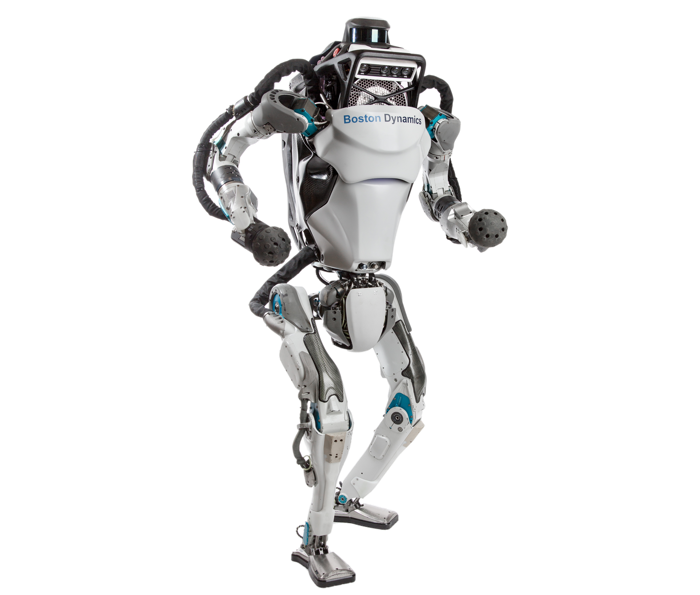
\includegraphics[scale=0.25]{atlas-page.png}\vspc

\large
 \begin{itemize}

	\item Review ODE45 Function\vspace{4mm}\\
	\item A Homework Problem \vspace{4mm}\\
	\item Solution Validation  \vspace{4mm}\\	
	\item MATLAB Solution\vspace{4mm}\\

\end{itemize}
%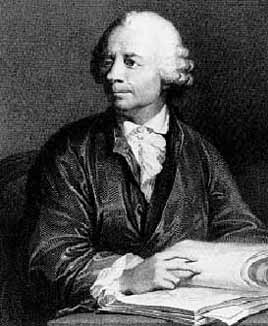
\includegraphics[scale=0.4]{euler01.jpg}\vspc
%\small Leonard Euler (1707-1783)
\end{multicols}
}


% Section 1 - Review ODE45 function
\section{Review ODE45 Function}
\subsection{Using the ODE45 Function}

\frame[containsverbatim]{

  \frametitle{Using the ODE45 Function}

 
The {\bf ode45} function is a MATLAB tool for solving differential \vspc equations. The equation(s) must be \underline{\hspace{20mm}-\hspace{25mm}}.

  \begin{framed}
  \begin{lstlisting}[numbers=none]
[TOUT,YOUT]=ode45(@ODEFUN,TSPAN,Y0,OPTS,P...);
  \end{lstlisting}
\end{framed}

%\vspace{0mm} Here is a description of the arguments.\vspace{1mm}\\

ODEFUN - name of the function containing the model \vspace{2mm}\\
TSPAN - time range for the initial value problem \vspace{2mm}\\
Y0 - initial value of the dependent variable \vspace{2mm}\\
OPTS - options defined by OPTIMSET function \vspace{2mm}\\
P... - additional parameters passed to ODEFUN \vspace{2mm}\\


}

\subsection{Euler's Method in MATLAB}
\frame[containsverbatim]{
  \frametitle{Euler's Method in MATLAB}

 \begin{lstlisting}
% validate the solution with ODE45
opts=optimset('Display','none');
[t45,v45]=ode45(@vdot_model,time,v0,opts,F,m,c);

% show a graph of the solution
figure(1); hold on
plot(time,vel,'ro');pause %analytical solution
plot(t45,v45,'b*')  %numerical solution

% Inline function definitions go at the bottom
function [vdot]=vdot_model(tin,vin,F,m,c)
    vdot=(F-c*vin)/m;
end

  \end{lstlisting}

}

% Section 2 - A Homework Problem
\section{A Homework Problem}
\subsection{First and Second Order Linear Systems}
\frame{

\frametitle{First and Second Order Linear Systems}
\begin{itemize}

\item First and second order linear models are frequently used  in science and engineering

\item Lets work one of the second order problems from the homework. Hopefully you see it could represent one of the physical systems. 

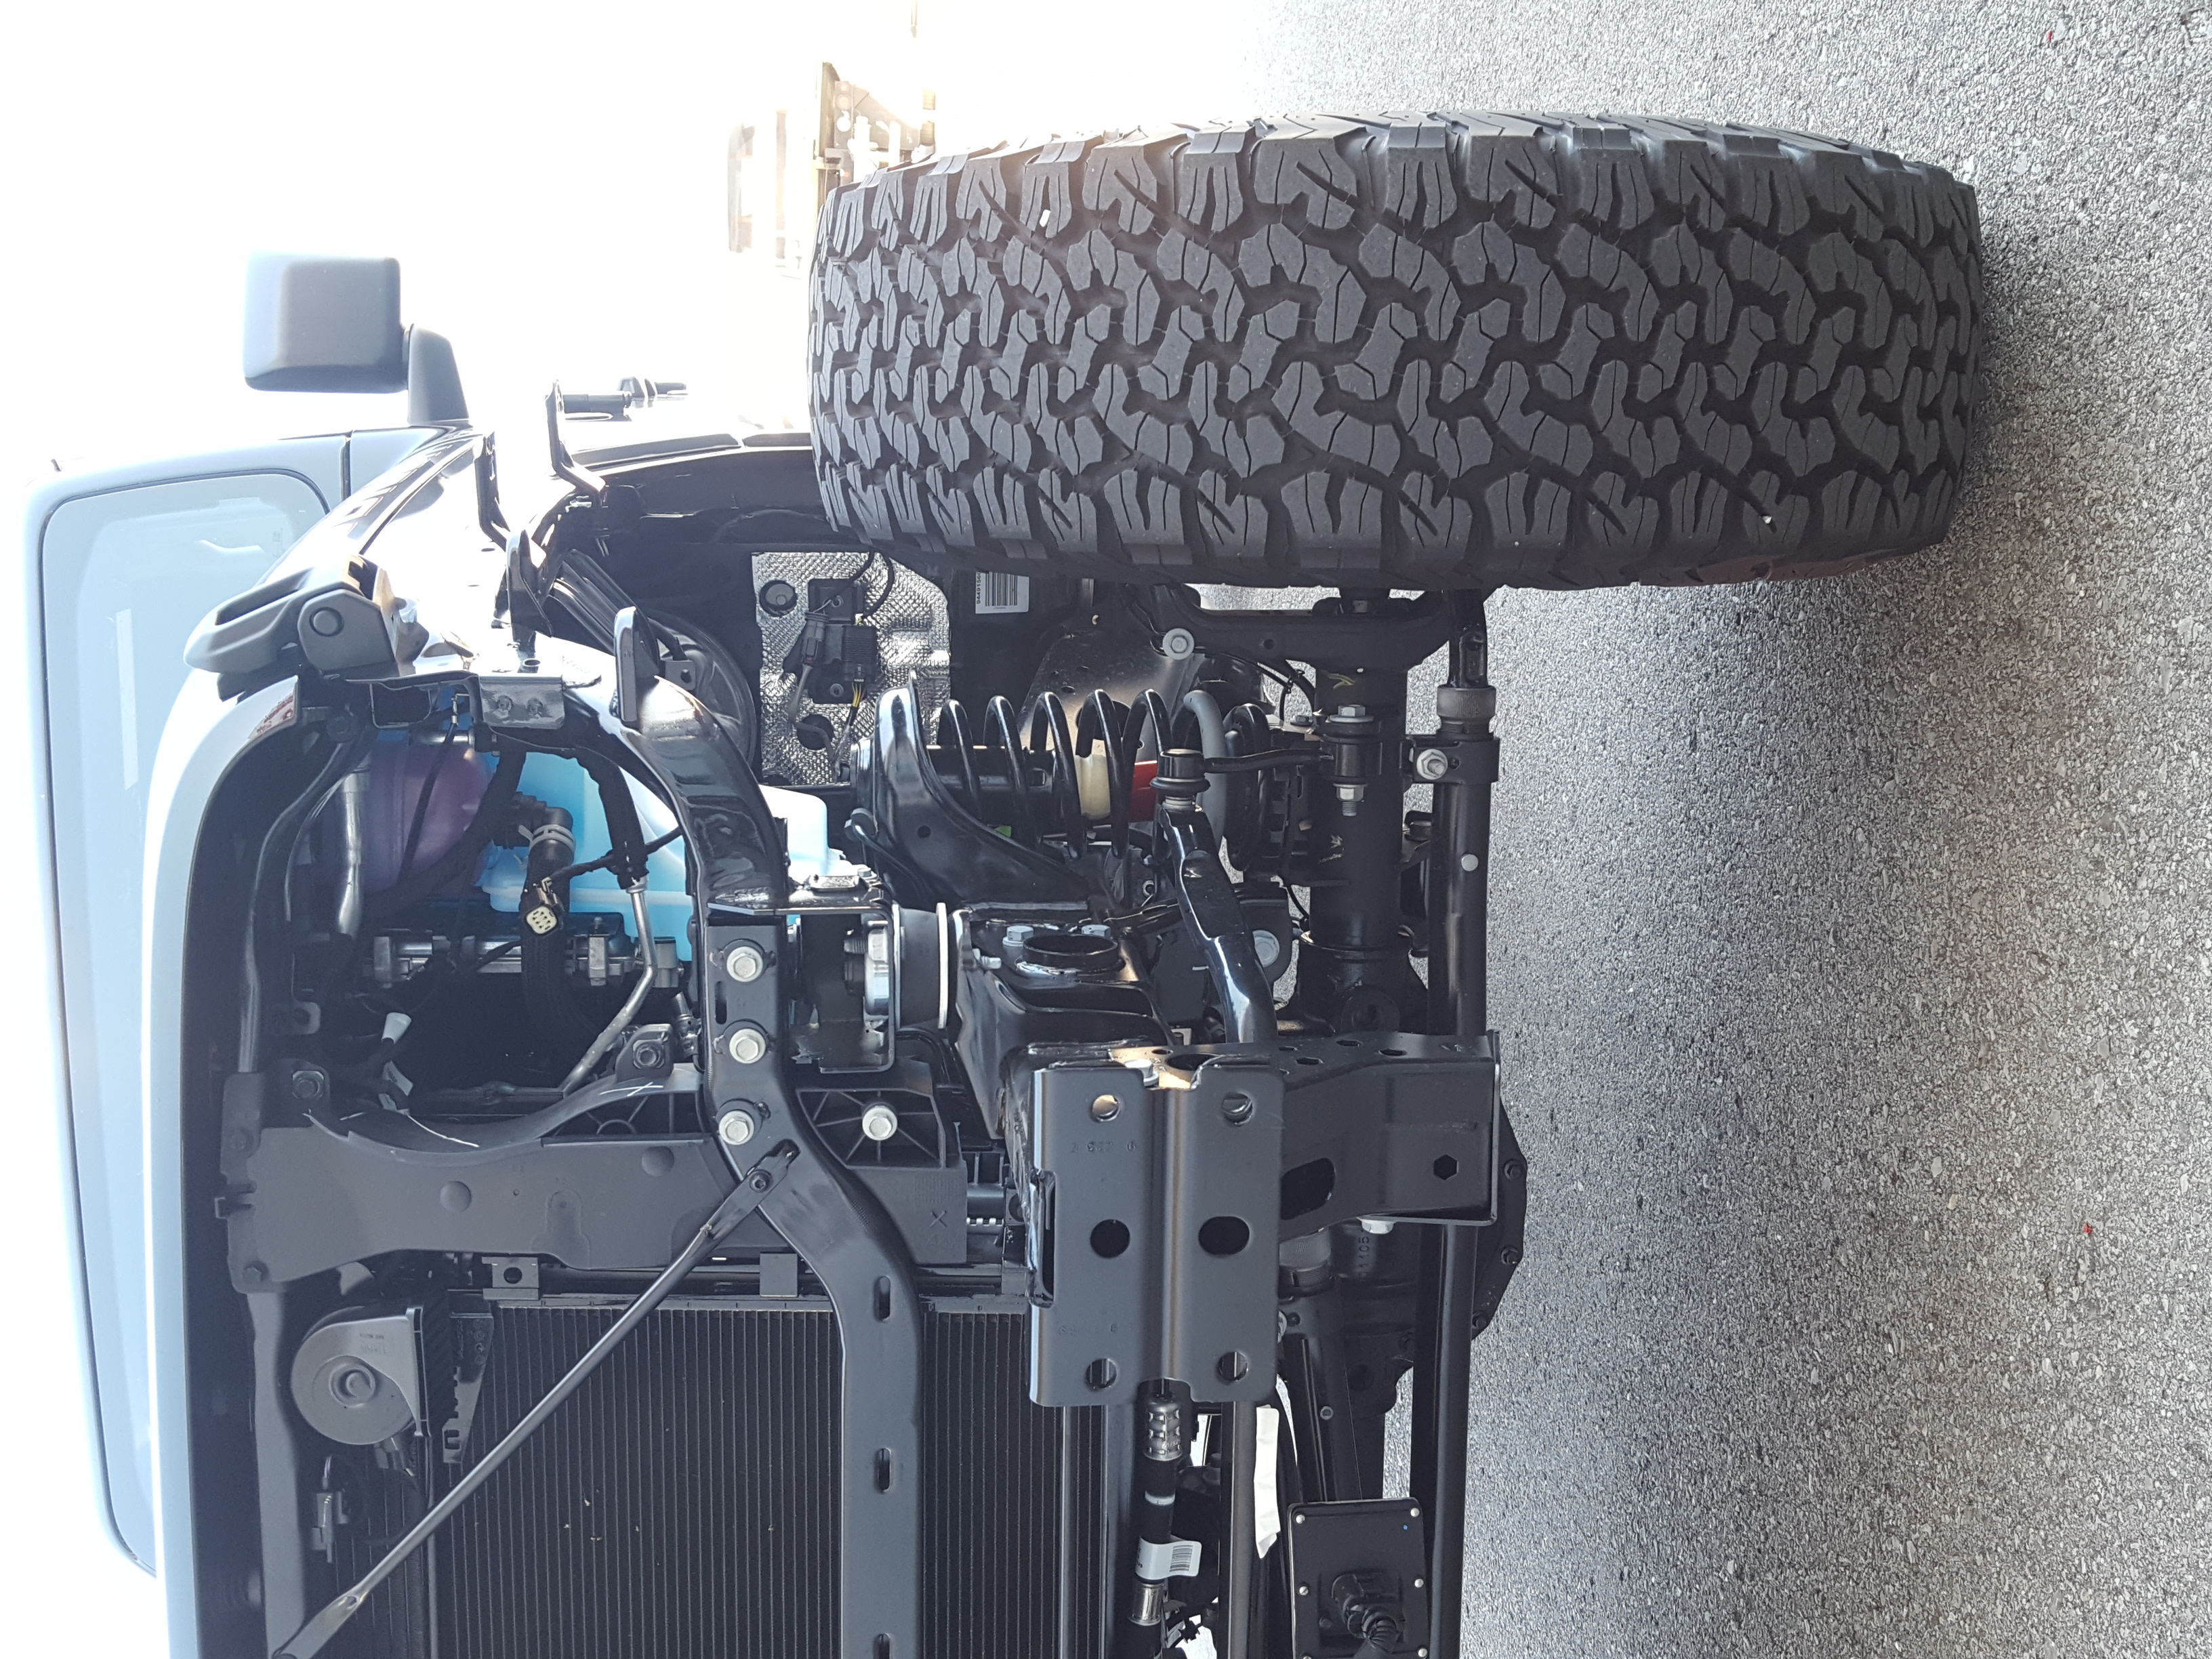
\includegraphics[scale=0.020,angle=-90,origin=c]{jeep_01.jpg}\hspace{10mm}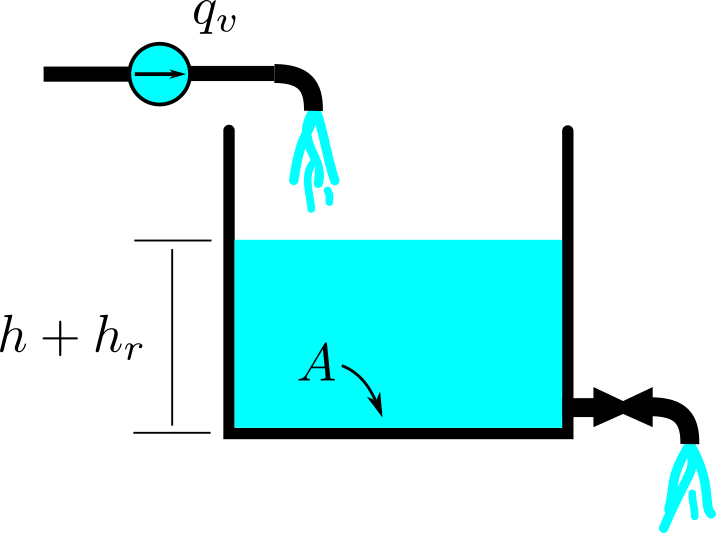
\includegraphics[scale=0.15]{water_tank.png}\hspace{10mm}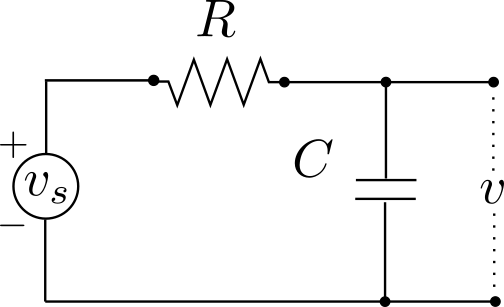
\includegraphics[scale=0.25]{rc_circuit.png}



\end{itemize}
}

\subsection{Homework 5 - Problem 1 Part C}
\frame{

\frametitle{Homework 5 - Problem 1 Part C plus a f(t)=6t}
\begin{framed}
Solve the following ODE using the trial solution method. \vspc
\scalebox{1}{$3\ddot{x}+12x=6t\hspccc \hspc x(0)=2\hspcc \dot{x}(0)=2$}
\end{framed}\vspace{5mm}
\underline{Step 1:} Find complementary part \vspccc
\underline{Step 2:} Find particular part		\vspccc
\underline{Step 3:} Combine and Solve for Unknown Constants \vspccc
\vspace{50mm}

}
\subsection{Find Complementary Solution}
\frame{

\frametitle{Find Complementary Solution}
\underline{Step 1:} Find complementary part from the LHS=0 of the ODE. \vspace{50mm}

}

\subsection{Find Particular Solution}
\frame{

\frametitle{Find Particular Solution}
\underline{Step 2:} Find particular part from the LHS=RHS of the ODE. \vspace{50mm}

}

\subsection{Combine and Solve for Unknown Constants}
\frame{

\frametitle{Combine and Solve for Unknown Constants}
\underline{Step 3:} The solution is the sum of the complementary and particular parts. Solve for the two remaining unknowns. \vspace{50mm}

}

\subsection{Analyitcal Solution}
\frame{

\frametitle{Analyitcal Solution}

\scalebox{1}{$x(t)=2cos(2t)+\frac{3}{4}sin(2t)+\frac{1}{2}t$} \vspace{50mm}

}


% Section 3 - Solution Validation
\section{Solution Validation}
\subsection{Equation Decomposition}
\frame{
As we have seen using ODE45 is not hard, but we have to setup the problem correctly. This is a re-occuring theme!!! \vspccc
\scalebox{1}{$3\ddot{x}+12x=6t\hspccc \hspc x(0)=2\hspcc \dot{x}(0)=2$} \vspcc

ODE45 can solve higher order equations but they must be written as a system of\underline{\hspace{15mm}}\hspace{3mm}\underline{\hspace{20mm}} \vspccc
There are two derivatives so there are two \underline{\hspace{15mm}}\hspace{3mm}\underline{\hspace{20mm}} \vspc differential equations \vspc
}


\subsection{x2 First Order from x1 Second Order}
\frame{

\frametitle{x2 First Order from x1 Second Order}

{\it One} second order ODE can be {\bf decomposed} into {\it two} first order ODEs through a simple change of variables.\vspccc

\scalebox{1}{$3\ddot{x}+12x=6t\hspccc \hspc x(0)=2\hspcc \dot{x}(0)=2$} \vspace{40mm}

}


\subsection{The ODE45 Function}
\frame[containsverbatim]{

\begin{lstlisting}[numbers=none,basicstyle=\ttfamily\tiny]
>> help ode45
 ode45  Solve non-stiff differential equations, medium order method.
    [TOUT,YOUT] = ode45(ODEFUN,TSPAN,Y0) with TSPAN = [T0 TFINAL] integrates 
    the system of differential equations y' = f(t,y) from time T0 to TFINAL 
    with initial conditions Y0. ODEFUN is a function handle. For a scalar T
    and a vector Y, ODEFUN(T,Y) must return a column vector corresponding 
    to f(t,y). Each row in the solution array YOUT corresponds to a time 
    returned in the column vector TOUT.  To obtain solutions at specific 
    times T0,T1,...,TFINAL (all increasing or all decreasing), use TSPAN = 
    [T0 T1 ... TFINAL].     
    
    [TOUT,YOUT] = ode45(ODEFUN,TSPAN,Y0,OPTIONS) solves as above with default
    integration properties replaced by values in OPTIONS, an argument created
    with the ODESET function. See ODESET for details. Commonly used options 
    are scalar relative error tolerance 'RelTol' (1e-3 by default) and vector
    of absolute error tolerances 'AbsTol' (all components 1e-6 by default).
    If certain components of the solution must be non-negative, use
    ODESET to set the 'NonNegative' property to the indices of these
    components.
\end{lstlisting}



}



% Section 4: MATLAB Solution
\section{MATLAB Solution}

\subsection{Part 1 - Program Setup}
\frame[containsverbatim]{
  \frametitle{Part 1 - Program Setup}



\begin{lstlisting}

clear variables;close all;clc

% create an array of time values
dt=.001;tstop=10;
t=0:dt:tstop;

% compute solution from derived equation
x_ex=2*cos(2*t)+3/4*sin(2*t)+1/2*t;
\end{lstlisting}

}

\subsection{Part 2 - Euler's Method}
\frame[containsverbatim]{
  \frametitle{Part 2 - Euler's Method}

% This method is not suitable for manual computation. \vspace{0mm}\\

 \begin{lstlisting}
% validate solution with ODE45
iv=[2 2];     % intitial vals for dependent var

opts=odeset('Stats','off');
[t_45,x_45]=ode45(@ode_sys,t,iv,opts);

% a function to use with ODE45
function [Zdot]=ode_sys(T,Z)  
    Zdot=zeros(2,1);
    Zdot(1)=Z(2);
    Zdot(2)=(5*T-12*Z(1))/3;
end
\end{lstlisting}

}

\subsection{Part 3 - Graph the Solutions}
\frame[containsverbatim]{
  \frametitle{Part 3 - Graph the Solutions}

% This method is not suitable for manual computation. \vspace{0mm}\\

 \begin{lstlisting}
% plot the results of the method
% plot the results of the method
figure(1);hold on
plot(t,x_ex,'r-','LineWidth',2)
plot(t_45,x_45(:,1),'b:','LineWidth',2)

grid on
str=sprintf('Solution to 3x''''+12x=6t, x(0)=2, x''(0)=2');
title(str)
legend('Analytical Solution','ODE45 Approximation')
xlabel('Time(s)');ylabel('x(t)')
  \end{lstlisting}

}


\frame[containsverbatim]{
\frametitle{ Do you believe the results?}

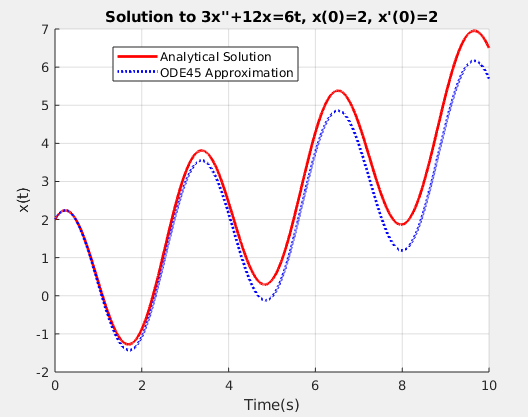
\includegraphics[scale=0.35]{lecture3_fig5.png}  \vspc
\small The graphs are close but they are not exactly the same! Why? \\
}


\end{document}


%\item \underline{ Differential Equations with Boundary Value Problems} - Zill 






